\documentclass[11pt,compress]{beamer}
\usepackage{ruc-research}
\title[个体投资者的信息集]{On the Information Set\\of Individual Investors}
\author[Laarits \& Wurgler]{Toomas Laarits\quad Jeffrey Wurgler}
\institute[NYU Stern]{NYU Stern School of Business}
\date{2026年4月27日工作稿}
\setbeamertemplate{page number in head/foot}{\insertframenumber/\inserttotalframenumber}
\begin{document}
\section{信息集为何重要}
% Physical page 01: 论文身份
\begin{frame}[plain]\titlepage\end{frame}
% Physical page 02: 行为资产定价中的信息输入问题
\begin{frame}{作者背景与论文定位}\relax
{\small\color{tsinghua}行为资产定价中的信息输入问题\par}\medskip
{\large\textbf{Jeffrey Wurgler　NYU Stern Nomura金融学讲席教授}}\par\medskip
{\small Baker–Wurgler情绪指标；Barberis–Shleifer–Wurgler《Comovement》}\par\medskip
{\small 曾任JFE、Management Science副编辑}\par\medskip
{\small Toomas Laarits　NYU Stern金融学助理教授}\par\medskip
{\small 2026-04-27工作稿；旧题Research Behavior；公开主页标注R\&R}\par\medskip
\source{作者主页与历年CV；NBER WP 33625；本地2026稿p.1。身份与状态核验：2026-11-17。}
\end{frame}
% Physical page 03: 信息集的测量，怎样成为资产定价的研究贡献？
\begin{frame}{本文的论证结构}\relax
{\small\color{tsinghua}信息集的测量，怎样成为资产定价的研究贡献？\par}\medskip
一 研究需要：理论的信息设定与可观察证据之间缺了什么\par\medskip
二 测量设计：跨平台URL怎样形成统一的研究与交易记录\par\medskip
三 四维证据：投入与主题 \(\rightarrow\) 股票与投资者差异 \(\rightarrow\) 交易时点与顺序\par\medskip
四 学术判断：贡献、局限、后续，以及汇报人的评价\par\medskip
\end{frame}
% Physical page 04: 公开信息怎样进入每一位投资者的决策？
\begin{frame}{信息获取是投资决策的起点}\relax
{\small\color{tsinghua}公开信息怎样进入每一位投资者的决策？\par}\medskip
Available information：市场可得的价格、新闻与公司资料\par
{\color{tsinghua}\(\downarrow\)}\par
\alert{Observed exposure：投资者实际访问的内容〔本文测量核心〕}\par
{\color{tsinghua}\(\downarrow\)}\par
Beliefs：加工信息，形成对收益与风险的判断\par
{\color{tsinghua}\(\downarrow\)}\par
Preferences / constraints：结合偏好、持仓与约束考虑行动\par
{\color{tsinghua}\(\downarrow\)}\par
Trade / portfolio：交易或组合选择\par
\source{原文pp.2–3；链条按研究对象整理。}
\end{frame}
% Physical page 05: 资产定价公式中的信息集，究竟为谁所知？
\begin{frame}{条件期望取决于信息条件}\relax
{\small\color{tsinghua}资产定价公式中的信息集，究竟为谁所知？\par}\medskip
\begin{equation*}P_t=\mathbb E_i[m_{i,t+1}(P_{t+1}+D_{t+1})\mid\mathcal I_{i,t}]\end{equation*}\medskip
价格评价同时依赖未来支付、贴现因子与条件信息集\par\medskip
相同公开信息环境，可以对应不同的个体信息条件\par\medskip
理性预期允许信息不同；同质预期还需额外共同条件\par\medskip
\source{讲解用条件定价关系，非本文估计式；原文pp.2–3。}
\end{frame}
% Physical page 06: 不同理论需要哪些可检验的信息输入事实？
\begin{frame}{模型的信息设定决定经济机制}\relax
{\small\color{tsinghua}不同理论需要哪些可检验的信息输入事实？\par}\medskip
组合选择：方差、协方差是否进入个体判断\par\medskip
噪声交易与情绪：哪些非基本面信号进入需求\par\medskip
信息扩散与收益外推：新闻与价格模式由谁处理\par\medskip
因此需要比较内容构成及其在人与股票之间的分布\par\medskip
\source{原文p.2：Markowitz、Sharpe、De Long等、Hong–Stein及外推模型。}
\end{frame}
% Physical page 07: 市场反映公开信息，是否意味着个人都处理了这些信息？
\begin{frame}{信息效率与个体信息集的距离}\relax
{\small\color{tsinghua}市场反映公开信息，是否意味着个人都处理了这些信息？\par}\medskip
有效市场讨论价格反映哪一类信息：历史价格、公开或私人信息\par\medskip
个体行为研究讨论谁接触什么，以及怎样形成需求\par\medskip
少数知情边际投资者可以参与价格发现；散户输入仍可能异质\par\medskip
测量个体信息集，补充市场效率与个体决策之间的微观环节\par\medskip
\source{原文pp.2–3、6–7；微观解释为汇报整理。}
\end{frame}
% Physical page 08: 知道一只股票受到关注，仍缺少什么？
\begin{frame}{已有注意力证据为何不够}\relax
{\small\color{tsinghua}知道一只股票受到关注，仍缺少什么？\par}\medskip
新闻、极端收益和搜索量：能观察注意力何时上升\par\medskip
但总量不能说明同一人看了价格、盈利还是风险\par\medskip
孤立代理难以放到共同分母下比较内容的相对重要性\par\medskip
本文需要把内容、投资者与交易同时连接起来\par\medskip
\source{原文pp.5–6；Barber–Odean（2008）、Da等（2011、2015）。}
\end{frame}
% Physical page 09: 最接近的点击流研究之后，本篇新增在哪里？
\begin{frame}{跨平台微观记录补上什么}\relax
{\small\color{tsinghua}最接近的点击流研究之后，本篇新增在哪里？\par}\medskip
单一券商点击流：可连接账户行为，但站外研究与细主题受限\par\medskip
本文跨券商和财经网站，减少单平台截断\par\medskip
URL参数给出股票、主题，时间戳连接先后与交易\par\medskip
研究单位能够下沉到家庭—股票—内容—时间\par\medskip
\source{原文p.3、pp.16–19；对照Gargano–Rossi（2018）。}
\end{frame}
% Physical page 10: 为什么不用一个注意力指数概括全部研究？
\begin{frame}{高维信息需要有组织地刻画}\relax
{\small\color{tsinghua}为什么不用一个注意力指数概括全部研究？\par}\medskip
同样十分钟，可以涉及不同股票、主题、来源与顺序\par\medskip
相同总量可能对应不同的信息集，也可能处于不同交易阶段\par\medskip
一条总指数会混合研究资源、内容偏向和参与者构成\par\medskip
作者选择四个互补维度，保留高维对象的关键结构\par\medskip
\source{原文p.4对high-dimensional process及四维设计的说明。}
\end{frame}
% Physical page 11: 测量设计怎样对应理论和行为研究的需要？
\begin{frame}{四个维度分别回答什么}\relax
{\small\color{tsinghua}测量设计怎样对应理论和行为研究的需要？\par}\medskip
{\small\renewcommand{\arraystretch}{1.12}
\begin{tabularx}{\linewidth}{@{}>{\hsize=1.680\hsize\linewidth=\hsize\raggedright\arraybackslash}X>{\hsize=0.660\hsize\linewidth=\hsize\raggedright\arraybackslash}X>{\hsize=0.660\hsize\linewidth=\hsize\raggedright\arraybackslash}X@{}}\toprule
\textbf{维度} & \textbf{直接问题} & \textbf{研究需要}\\
\midrule
Depth 投入 & 研究资源有多少 & 约束信息获取强度\\
Topics 内容 & 接触哪些主题 & 约束模型的信号输入\\
Heterogeneity 差异 & 哪些股票、哪些人不同 & 刻画信息集分布\\
Timing 时点 & 何时、依次怎样研究 & 连接信息获取与行动\\
\bottomrule\end{tabularx}}
\medskip
\source{原文pp.4–7；研究需要为汇报整理。}
\end{frame}
% Physical page 12: 这套测量带来了怎样的新事实？
\begin{frame}{答案预览：选择性与异质性}\relax
{\small\color{tsinghua}这套测量带来了怎样的新事实？\par}\medskip
投入有限：已交易标的研究的家庭中位数约6分钟 / 次交易\par\medskip
内容不均：价格图突出，分析师较常见，风险统计专门访问少\par\medskip
风格有别：总体参与程度与快慢信息取向需要区分\par\medskip
临近交易集中：许多路径只涉及少数保留主题\par\medskip
\source{2026稿Tables 2–5、Figures 3–5；6分钟约数对应5.7。}
\end{frame}
% Physical page 13: 什么样的信息假设因此更有现实依据？
\begin{frame}{这些事实怎样约束资产定价}\relax
{\small\color{tsinghua}什么样的信息假设因此更有现实依据？\par}\medskip
价格输入突出：历史窗口与平台默认应进入信念模型的设定\par\medskip
个体差异明显：共同信息或代表性主体可能遗漏重要结构\par\medskip
风险指标专门访问少：不能直接把规范参数当作散户研究过程\par\medskip
经验贡献是约束模型输入；价格效应仍需需求与均衡证据\par\medskip
\source{原文pp.6–7、40–41。}
\end{frame}
% Physical page 14: 内容侧重来自偏好，还是成本与平台供给？
\begin{frame}{信息获取也是内生选择}\relax
{\small\color{tsinghua}内容侧重来自偏好，还是成本与平台供给？\par}\medskip
投入取决于预期决策价值与获取、处理成本\par\medskip
平台默认影响最先接触的内容及额外搜索成本\par\medskip
标的特征可能同时改变信息供给与投资者需求\par\medskip
因此依次研究内容、股票特征与个体风格，而不提前选定机制\par\medskip
\source{据原文pp.26–36作经济解释，非本文结构模型。}
\end{frame}
% Physical page 15: 四维问题如何落到可分析的数据对象？
\begin{frame}{同一份明细支持三层比较}\relax
{\small\color{tsinghua}四维问题如何落到可分析的数据对象？\par}\medskip
底层：家庭 i × 股票 j × 主题 k × 时间 t 的研究记录\par\medskip
家庭层：投入与主题配置，回答一个投资者拥有什么输入\par\medskip
股票层：股票—月份回归，回答哪些标的吸引何种研究\par\medskip
事件层：家庭—股票—交易与搜索路径，回答研究怎样接近行动\par\medskip
\source{据原文各节观测单位整理；不是额外估计模型。}
\end{frame}
\section{如何构造测量}
% Physical page 16: 怎样把原始浏览流变成能回答四维问题的数据？
\begin{frame}{预处理的目标是统一研究与交易记录}\relax
{\small\color{tsinghua}怎样把原始浏览流变成能回答四维问题的数据？\par}\medskip
输入：家庭标识、时间戳、页面活动时间、原始URL\par\medskip
研究流：域名与参数 \(\rightarrow\) 股票 / 主题 \(\rightarrow\) 时间分配\par\medskip
交易流：订单语法与上下文 \(\rightarrow\) 股票 / 方向 \(\rightarrow\) 合并重复记录\par\medskip
输出：研究明细 (i,j,k,t,\(\Delta\)t) 与交易事件 (i,j,t*,方向)\par\medskip
\source{Internet Appendix Steps 1–10，pp.58–68。}
\end{frame}
% Physical page 17: 最清楚的URL怎样形成一行研究数据？
\begin{frame}{案例一：专门页面直接识别主题}\relax
{\small\color{tsinghua}最清楚的URL怎样形成一行研究数据？\par}\medskip
输入：http://finance.yahoo.com/q/ao?s=IMCL\par\medskip
域名确定信息来源；s=IMCL确定股票；ao需历史页面核验\par\medskip
核验后：analyst opinions \(\rightarrow\) 分析师信息；保留该次活动时间\par\medskip
输出：(家庭 i，IMCL，Analysts，时间 t，活动时长 \(\Delta\)t)\par\medskip
\source{原文p.10；Internet Appendix Step 3，p.61。}
\end{frame}
% Physical page 18: 同一URL含多种信息，怎样避免重复计算研究时间？
\begin{frame}{案例二：复合图表必须拆分}\relax
{\small\color{tsinghua}同一URL含多种信息，怎样避免重复计算研究时间？\par}\medskip
输入：earnings/update\_earningsChart.asp?…indicator=volume,1,13,EMA,13\par\medskip
参数：duration=1095；daysforward=545；year=2006\par\medskip
识别：约3年历史盈利、约1.5年前瞻；附成交量 / 移动平均信息\par\medskip
输出：按可识别主题拆分，分配后的时长合计仍为原时长 \(\Delta\)t\par\medskip
\source{原文p.10；Internet Appendix Step 4，pp.62–63。URL参数为原文示例。}
\end{frame}
% Physical page 19: 订单流怎样成为交易事件，研究时间又怎样归属？
\begin{frame}{交易识别使研究能够对齐行动}\relax
{\small\color{tsinghua}订单流怎样成为交易事件，研究时间又怎样归属？\par}\medskip
订单URL：ordertype="sell" \& symbol=GOOG \& shares=100\par\medskip
结合上下文核验；同股票同方向、间隔\(\le\)30分钟合为一次\par\medskip
研究流按家庭—股票连接交易；两次同股交易间研究归给下一笔\par\medskip
无后续交易则记为交易后；15分钟浏览会话不是交易去重阈值\par\medskip
\source{Internet Appendix pp.59–60；研究归属见原文p.37。此例按URL明示为卖出。}
\end{frame}
% Physical page 20: 哪些规则必须保留，哪些只是程序细节？
\begin{frame}{分类与匹配保护什么含义}\relax
{\small\color{tsinghua}哪些规则必须保留，哪些只是程序细节？\par}\medskip
{\small\renewcommand{\arraystretch}{1.12}
\begin{tabularx}{\linewidth}{@{}>{\hsize=0.740\hsize\linewidth=\hsize\raggedright\arraybackslash}X>{\hsize=1.260\hsize\linewidth=\hsize\raggedright\arraybackslash}X@{}}\toprule
\textbf{处理选择} & \textbf{保护的统计含义}\\
\midrule
同一单一ticker前后夹定才补配 & 减少把新闻错归给其他股票\\
研究与持仓 / 订单 / 银行业务分开 & 投入只统计信息研究\\
Snapshot保留原分类，另作内容归因 & 区分页面接触与推算的内容时间\\
484户总量；50户高匹配率动态 & 匹配精度服务于相应研究问题\\
\bottomrule\end{tabularx}}
\medskip
\source{原文pp.18–24；Internet Appendix Steps 6、8、10。}
\end{frame}
% Physical page 21: 统一输出之后，分别聚合成哪些观测？
\begin{frame}{样本与分析层级}\relax
{\small\color{tsinghua}统一输出之后，分别聚合成哪些观测？\par}\medskip
{\small\renewcommand{\arraystretch}{1.12}
\begin{tabularx}{\linewidth}{@{}>{\hsize=0.740\hsize\linewidth=\hsize\raggedright\arraybackslash}X>{\hsize=1.260\hsize\linewidth=\hsize\raggedright\arraybackslash}X@{}}\toprule
\textbf{层级} & \textbf{观测与用途}\\
\midrule
原始样本 & 484户；2,911笔；2007年1、2、3、6月\\
家庭×主题 & 月参与、研究分钟 / 次交易；投入与配置\\
股票×月份 & 市值前1,000只；3,962行；研究覆盖与内容\\
家庭×股票×交易 / 路径 & 50户精确时间；484户可识别主题路径\\
\bottomrule\end{tabularx}}
\medskip
\source{原文Tables 1–5、Figures 3–5；家庭而非自然人。}
\end{frame}
\section{四维研究证据}
% Physical page 22: 投入：典型投资者与研究右尾需要同时观察
\begin{frame}{维度一：研究资源有多少}\relax
{\small\color{tsinghua}投入：典型投资者与研究右尾需要同时观察\par}\medskip
{\small\renewcommand{\arraystretch}{1.12}
\begin{tabularx}{\linewidth}{@{}>{\hsize=1.720\hsize\linewidth=\hsize\raggedright\arraybackslash}X>{\hsize=0.760\hsize\linewidth=\hsize\raggedright\arraybackslash}X>{\hsize=0.760\hsize\linewidth=\hsize\raggedright\arraybackslash}X>{\hsize=0.760\hsize\linewidth=\hsize\raggedright\arraybackslash}X@{}}\toprule
\textbf{范围} & \textbf{样本} & \textbf{均值} & \textbf{中位数}\\
\midrule
全部标的 & 484户 & 144.2 & 36.4\\
全部标的 & 50户 & 96.8 & 51.7\\
实际交易标的 & 50户 & 29.1 & 5.7\\
\bottomrule\end{tabularx}}
\medskip
家庭内先算研究分钟 / 交易次数，再在家庭之间统计\par\medskip
全部研究与已交易标的研究的差异，说明大量研究没有当期交易\par\medskip
均值远高于中位数；站外研究对均值投资者超过一半\par\medskip
\source{据原文Table 2 Panels B–C，p.47。不是逐笔交易时长分布。}
\end{frame}
% Physical page 23: 内容：相同的研究总量，可能形成不同的信息集
\begin{frame}{维度二：信息资源配置到了哪里}\relax
{\small\color{tsinghua}内容：相同的研究总量，可能形成不同的信息集\par}\medskip
{\small\renewcommand{\arraystretch}{1.12}
\begin{tabularx}{\linewidth}{@{}>{\hsize=1.680\hsize\linewidth=\hsize\raggedright\arraybackslash}X>{\hsize=0.660\hsize\linewidth=\hsize\raggedright\arraybackslash}X>{\hsize=0.660\hsize\linewidth=\hsize\raggedright\arraybackslash}X@{}}\toprule
\textbf{原始页面类别} & \textbf{曾访问的家庭比例} & \textbf{均值分钟 / 次交易}\\
\midrule
价格图表 & 93\% & 39.1\\
综合行情 & 93\% & 37.0\\
分析师信息 & 71\% & 12.5\\
其他基本面 & 53\% & 2.6\\
盈利 & 40\% & 1.7\\
风险统计 & 约1\%〔7户〕 & 四舍五入为0.0\\
\bottomrule\end{tabularx}}
\medskip
直接分类先比较专门访问；混合页归因用于补全内容总账\par\medskip
\source{据Table 3左侧原始分类摘录，p.48；7户见p.24。全样本、所有标的。}
\end{frame}
% Physical page 24: 内容：综合行情不能被直接当作一种单一经济信号
\begin{frame}{混合页归因如何影响内容比较}\relax
{\small\color{tsinghua}内容：综合行情不能被直接当作一种单一经济信号\par}\medskip
{\small\renewcommand{\arraystretch}{1.12}
\begin{tabularx}{\linewidth}{@{}>{\hsize=0.740\hsize\linewidth=\hsize\raggedright\arraybackslash}X>{\hsize=1.260\hsize\linewidth=\hsize\raggedright\arraybackslash}X@{}}\toprule
\textbf{对象} & \textbf{处理方式}\\
\midrule
Snapshot综合行情 & 历史页面核验；等权 / 展示比例 / 兴趣加权\\
主表的Snapshot口径 & 按全样本专门类别的参与兴趣加权\\
内容不明的新闻 & 部分券商标题、日期、股票与RavenPack匹配\\
内容不明的讨论板 & 按当代Reddit r/stocks的主题构成估计\\
顺序分析 Figures 4–5 & 保留Snapshot等原始页面，不作主题归因\\
\bottomrule\end{tabularx}}
\medskip
\source{Table 3；Internet Appendix Step 10，pp.66–68、Table IA2。}
\end{frame}
% Physical page 25: 内容：默认展示决定实际接触历史的重要部分
\begin{frame}{价格历史为何以短窗口为主}\relax
{\small\color{tsinghua}内容：默认展示决定实际接触历史的重要部分\par}\medskip
\centering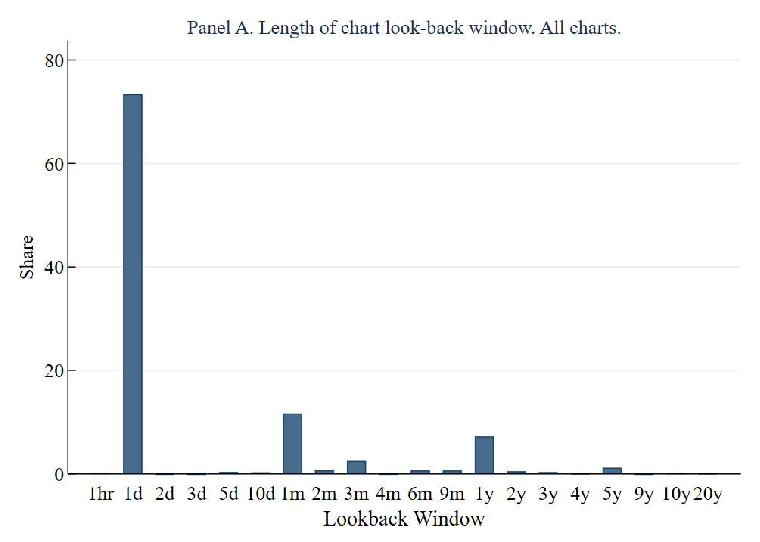
\includegraphics[width=\linewidth,height=4.46cm,keepaspectratio]{assets/chart_all.pdf}\par
{\small 含默认展示：超过70\%的可观察图表为日内窗口\par}
{\small 主动切换时更常选择一月至一年〔Figure 1B〕\par}
{\small 实际曝光与主动偏好共同决定观察到的价格输入\par}
\source{原文Figure 1 Panel A，p.52；解释见pp.26–27。原图。}
\end{frame}
% Physical page 26: 内容：规范风险参数是否表现为散户主动研究对象
\begin{frame}{低风险统计访问怎样解释}\relax
{\small\color{tsinghua}内容：规范风险参数是否表现为散户主动研究对象\par}\medskip
直接识别：484户中仅7户显示beta / 波动率的专门兴趣\par\medskip
加入混合页归因：均值1.8分钟 / 次交易，约占1.2\%\par\medskip
价格波动与经验也可能传递风险信息\par\medskip
理论含义：散户主动收集标准风险参数的假设需要事实支持\par\medskip
\source{原文pp.24–25、Table 3，p.48。1.2\%据1.8 / 144.2计算。}
\end{frame}
% Physical page 27: 信息配置差异来自标的，还是来自研究者？
\begin{frame}{维度三：先比较股票，再比较人}\relax
{\small\color{tsinghua}信息配置差异来自标的，还是来自研究者？\par}\medskip
股票×月份：相同标的在多少人中引起研究，研究什么内容\par\medskip
家庭×主题：不同家庭是否持续采取不同的研究侧重\par\medskip
两层比较互补：同一种总体内容结构可以由不同机制形成\par\medskip
\source{原文Sections V–VI，pp.29–36。}
\end{frame}
% Physical page 28: 股票层面：覆盖广度、总量与内容配置如何分别测量？
\begin{frame}{三个因变量对应三个不同问题}\relax
{\small\color{tsinghua}股票层面：覆盖广度、总量与内容配置如何分别测量？\par}\medskip
\begin{equation*}A_{jm}=\frac{100}{N_m}\sum_i\mathbf1(T_{ijm}>0)\end{equation*}\medskip
A：研究该股的人数比例，衡量关注覆盖广度\par\medskip
L = ln(1 + 总研究分钟)，同时包含人数与深度\par\medskip
D = A价格 - A基本面，衡量内容关注的相对广度\par\medskip
同一人可进入两类内容，D并非互斥人群或时间占比\par\medskip
\source{按Table 4表注定义整理，pp.49–50；符号为汇报重写。}
\end{frame}
% Physical page 29: 如何把关注差异与股票特征关联起来？
\begin{frame}{股票月份回归的比较与规格}\relax
{\small\color{tsinghua}如何把关注差异与股票特征关联起来？\par}\medskip
\begin{equation*}Y_{jm}=\alpha+\beta\,z(\ln MC_{jm})+\gamma^{\prime}Z_{jm}+\delta_{\mathrm{FF49}(j)}+\varepsilon_{jm}\end{equation*}\medskip
Y分别取A、L或D；一行是股票—月份，N=3,962\par\medskip
Z：规模、新闻、风险、历史收益等；非虚拟变量标准化\par\medskip
扩展规格加入FF49行业效应与散户交易 / 持有变量\par\medskip
系数来自条件相关；原表采用滞后2个月Newey–West标准误\par\medskip
\source{按2026稿Table 4列1–6重写；行业效应在扩展列加入。}
\end{frame}
% Physical page 30: 股票：先解释关注人数，再讨论内容侧重
\begin{frame}{规模主要解释谁进入研究集合}\relax
{\small\color{tsinghua}股票：先解释关注人数，再讨论内容侧重\par}\medskip
{\small\renewcommand{\arraystretch}{1.12}
\begin{tabularx}{\linewidth}{@{}>{\hsize=1.120\hsize\linewidth=\hsize\raggedright\arraybackslash}X>{\hsize=0.720\hsize\linewidth=\hsize\raggedright\arraybackslash}X>{\hsize=1.080\hsize\linewidth=\hsize\raggedright\arraybackslash}X>{\hsize=1.080\hsize\linewidth=\hsize\raggedright\arraybackslash}X@{}}\toprule
\textbf{关注覆盖广度} & \textbf{第1列} & \textbf{第2列} & \textbf{第3列}\\
\midrule
标准化 ln市值 & 1.03*** & 1.33*** & 1.13***\\
t值 & 14.42 & 13.57 & 11.35\\
扩展控制 & 仅市值 & 加特征与行业 & 再加散户变量\\
\(R^2\) & 0.315 & 0.447 & 0.484\\
\bottomrule\end{tabularx}}
\medskip
一个标准差：覆盖比例约1.01\% \(\rightarrow\) 2.04\%，增加1.03个百分点\par\medskip
\(R^2\)从0.315到0.484描述样本变异解释度，不是因果效应\par\medskip
\source{据Table 4列1–3摘录，pp.49–50；N=3,962。*** p<0.01；t值为原表。}
\end{frame}
% Physical page 31: 股票：下跌后的监控需求，也可能带来更多研究
\begin{frame}{风险与历史收益如何关联总关注}\relax
{\small\color{tsinghua}股票：下跌后的监控需求，也可能带来更多研究\par}\medskip
{\small\renewcommand{\arraystretch}{1.12}
\begin{tabularx}{\linewidth}{@{}>{\hsize=1.800\hsize\linewidth=\hsize\raggedright\arraybackslash}X>{\hsize=0.660\hsize\linewidth=\hsize\raggedright\arraybackslash}X>{\hsize=0.540\hsize\linewidth=\hsize\raggedright\arraybackslash}X@{}}\toprule
\textbf{研究覆盖比例，第3列} & \textbf{系数〔百分点〕} & \textbf{t值}\\
\midrule
收益波动率 & 0.09*** & 2.80\\
财报月份〔0/1〕 & 0.26*** & 5.21\\
前一个月收益 & -0.08*** & -2.92\\
动量收益〔t-2至t-12〕 & -0.07** & -2.23\\
散户成交量份额 & 0.34*** & 6.24\\
\bottomrule\end{tabularx}}
\medskip
\source{据Table 4列3摘录，pp.49–50；其余控制同原表。*** p<0.01，** p<0.05。}
\end{frame}
% Physical page 32: 获得关注较多，与相对偏向价格研究是否相同？
\begin{frame}{内容之差为何提供额外信息}\relax
{\small\color{tsinghua}获得关注较多，与相对偏向价格研究是否相同？\par}\medskip
\begin{equation*}D_{jm}=A^{\mathrm{Price}}_{jm}-A^{\mathrm{Fundamentals}}_{jm}\end{equation*}\medskip
价格组：Price Charts + Technical\par\medskip
基本面组：盈利 + 分红 + 其他基本面 + 分析师 + 公司网站\par\medskip
先分别统计参与者比例，再相减；D>0表示价格覆盖更广\par\medskip
用D回归，可检视规模、风险与动量是否改变内容构成\par\medskip
\source{Table 4表注及原文p.32；按类别并集统计。}
\end{frame}
% Physical page 33: 股票：关注规模与信息构成的经济含义不同
\begin{frame}{高波动与动量更偏向价格研究}\relax
{\small\color{tsinghua}股票：关注规模与信息构成的经济含义不同\par}\medskip
{\small\renewcommand{\arraystretch}{1.12}
\begin{tabularx}{\linewidth}{@{}>{\hsize=1.800\hsize\linewidth=\hsize\raggedright\arraybackslash}X>{\hsize=0.660\hsize\linewidth=\hsize\raggedright\arraybackslash}X>{\hsize=0.540\hsize\linewidth=\hsize\raggedright\arraybackslash}X@{}}\toprule
\textbf{价格研究比例 - 基本面研究比例} & \textbf{第6列系数} & \textbf{t值}\\
\midrule
收益波动率 & 0.06*** & 4.63\\
动量收益〔t-2至t-12〕 & 0.05** & 2.33\\
分析师覆盖数 & -0.10** & -2.42\\
ln名义价格 & -0.09* & -1.72\\
ln市值 & 0.03 & 0.61\\
\bottomrule\end{tabularx}}
\medskip
波动率、动量正系数；分析师覆盖负系数\par\medskip
规模对总覆盖很重要，在内容之差中却不显著\par\medskip
两个因变量的不同方向，说明不能用“关注更多”替代内容分析\par\medskip
\source{据Table 4列6摘录，pp.49–50；N=3,962；*** p<0.01，** p<0.05，* p<0.10。}
\end{frame}
% Physical page 34: 股票：微观面板能否捕捉公共信息事件？
\begin{frame}{事件比较检验注意力的时间变化}\relax
{\small\color{tsinghua}股票：微观面板能否捕捉公共信息事件？\par}\medskip
\centering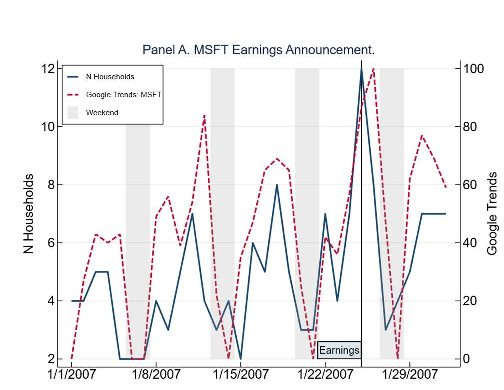
\includegraphics[width=\linewidth,height=4.46cm,keepaspectratio]{assets/event_msft.pdf}\par
{\small 财报附近：参与研究人数与Google搜索强度共同上升\par}
{\small 两者量纲不同；点击流还能追踪投资者与具体内容\par}
\source{原文Figure 2 Panel A，p.53；解释见pp.32–33。原图，左右轴含义不同。}
\end{frame}
% Physical page 35: 家庭层面：研究参与和研究什么股票如何共同变化？
\begin{frame}{PCA把研究习惯与标的倾向放在一起}\relax
{\small\color{tsinghua}家庭层面：研究参与和研究什么股票如何共同变化？\par}\medskip
\begin{equation*}X_i=\big(\mathbf1\{T_{i1}/M_i>2\},\ldots,\mathbf1\{T_{i,13}/M_i>2\},S_i\big)\end{equation*}\medskip
一行是一户家庭：13个主题的月研究时间是否超过2分钟\par\medskip
再加连续标的倾向S：高波动、小、年轻、低价等投机特征\par\medskip
加入S的目的：联系研究习惯与股票类型，而非只按信息类别分组\par\medskip
输入以阈值指标为主，反映参与；S精确权重未充分披露\par\medskip
\source{原文p.35、Table 5，p.51；风险统计因过少而排除。}
\end{frame}
% Physical page 36: 家庭：研究广度与标的投机倾向并非同一个维度
\begin{frame}{PC1概括总体研究参与程度}\relax
{\small\color{tsinghua}家庭：研究广度与标的投机倾向并非同一个维度\par}\medskip
{\small\renewcommand{\arraystretch}{1.12}
\begin{tabularx}{\linewidth}{@{}>{\hsize=1.400\hsize\linewidth=\hsize\raggedright\arraybackslash}X>{\hsize=0.600\hsize\linewidth=\hsize\raggedright\arraybackslash}X@{}}\toprule
\textbf{变量〔摘录〕} & \textbf{PC1载荷}\\
\midrule
News–Indeterminate & 0.36\\
Snapshot / Analysts & 0.32 / 0.32\\
Price Chart & 0.31\\
Other Fundamentals & 0.28\\
Speculative Stock Focus & 0.01\\
\bottomrule\end{tabularx}}
\medskip
特征值3.75；解释变异26.81\%\par\medskip
输入多为阈值指标：更适合解释为总体参与程度\par\medskip
\source{据Table 5摘录，p.51。未列其余载荷；主成分整体符号可翻转。}
\end{frame}
% Physical page 37: 家庭：载荷怎样连接研究习惯与标的倾向？
\begin{frame}{PC2概括快慢信息的侧重}\relax
{\small\color{tsinghua}家庭：载荷怎样连接研究习惯与标的倾向？\par}\medskip
{\small\renewcommand{\arraystretch}{1.12}
\begin{tabularx}{\linewidth}{@{}>{\hsize=1.520\hsize\linewidth=\hsize\raggedright\arraybackslash}X>{\hsize=0.480\hsize\linewidth=\hsize\raggedright\arraybackslash}X>{\hsize=1.520\hsize\linewidth=\hsize\raggedright\arraybackslash}X>{\hsize=0.480\hsize\linewidth=\hsize\raggedright\arraybackslash}X@{}}\toprule
\textbf{正向 / 近零变量} & \textbf{PC2} & \textbf{负向变量} & \textbf{PC2}\\
\midrule
Message Board & 0.46 & Dividends & -0.47\\
Speculative Stock Focus & 0.43 & Earnings & -0.34\\
Snapshot & 0.30 & Other Fundamentals & -0.29\\
Price Chart & 0.19 & Technical & -0.11\\
Analysts & 0.00 & Ownership & -0.18\\
\bottomrule\end{tabularx}}
\medskip
PC2解释8.77\%；PC1 + PC2合计35.58\%\par\medskip
投机指标参与构造，载荷描述共变，不能解释因果方向\par\medskip
\source{据Table 5摘录，p.51；未列其余近零载荷。整体符号可翻转。}
\end{frame}
% Physical page 38: 时点：研究集中程度比买卖总量差异更突出
\begin{frame}{维度四：有限研究何时发生}\relax
{\small\color{tsinghua}时点：研究集中程度比买卖总量差异更突出\par}\medskip
\begin{columns}[c]\begin{column}{.51\textwidth}\centering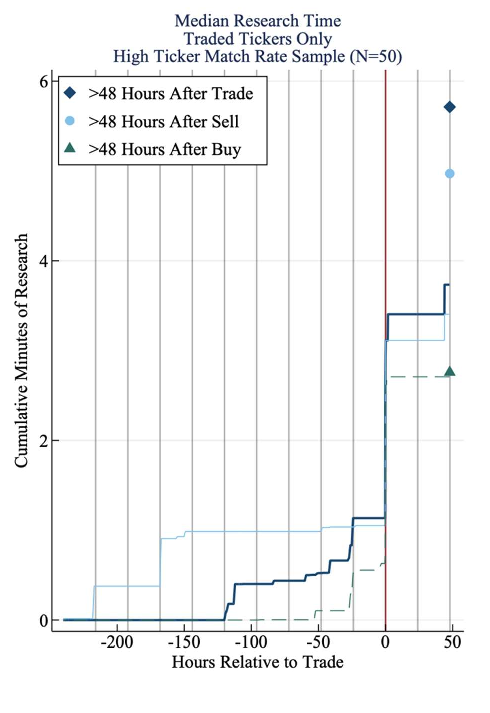
\includegraphics[width=\linewidth,height=5.1cm,keepaspectratio]{assets/timing_median.pdf}\end{column}\begin{column}{.44\textwidth}
50户高匹配率样本，家庭内先按交易平均\par\medskip
中位数研究在临近交易时迅速累积；买入前更集中\par\medskip
这里刻画发生时间，不能定位交易意向最初形成的时刻\par\medskip
\end{column}\end{columns}
\source{原文Figure 3右面板，p.54；解释见pp.37–38。原图。}
\end{frame}
% Physical page 39: 相同内容总量，是否意味着相同的信息获取过程？
\begin{frame}{为何还需要研究主题顺序}\relax
{\small\color{tsinghua}相同内容总量，是否意味着相同的信息获取过程？\par}\medskip
静态分类丢失顺序：先价格后盈利，与先盈利后价格可以同量\par\medskip
同户同股合并10天；重复主题只保留首次，Snapshot不归因\par\medskip
价格 \(\rightarrow\) 盈利 \(\rightarrow\) 分红 \(\rightarrow\) 价格，压缩为价格 \(\rightarrow\) 盈利 \(\rightarrow\) 分红 \(\rightarrow\) END\par\medskip
图另省略少数类别；路径长度指保留主题数，不是点击数\par\medskip
\source{原文pp.38–39、Figures 4–5图注；序列为原文示例。}
\end{frame}
% Physical page 40: 顺序：研究往往在哪一类信息后停止？
\begin{frame}{入口与终止：综合行情的关键位置}\relax
{\small\color{tsinghua}顺序：研究往往在哪一类信息后停止？\par}\medskip
\centering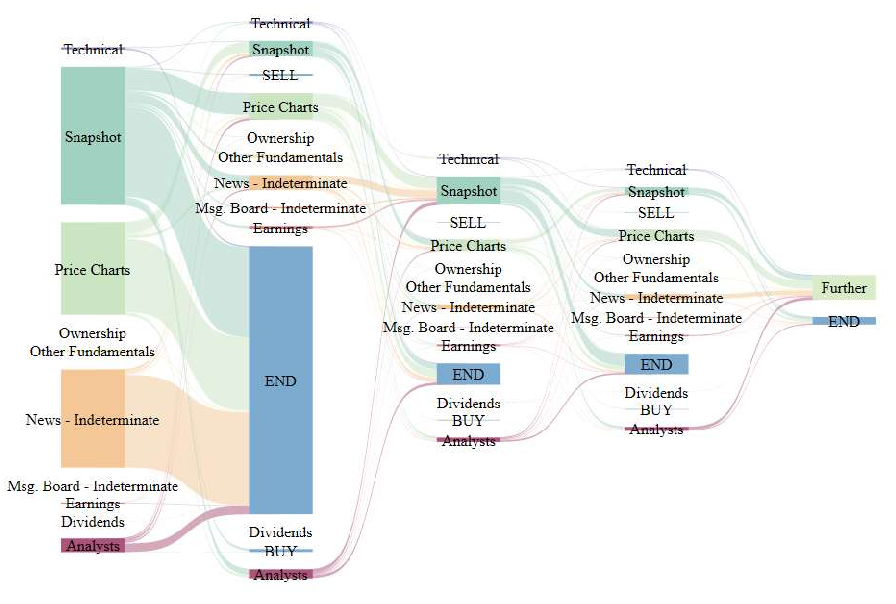
\includegraphics[width=\linewidth,height=3.65cm,keepaspectratio]{assets/paths.pdf}\par
{\small 从左向右：首次、第二个及后续保留主题；END为结束\par}
{\small 线宽是合并研究窗口数，BUY / SELL标记交易\par}
{\small Snapshot常作入口；许多路径在一个保留主题后结束\par}
\source{原文Figure 4，p.55；484户、16,930条路径；解释见pp.38–39。原图。}
\end{frame}
% Physical page 41: 给定交易后的路径，能否说明信息触发了行动？
\begin{frame}{交易条件与风格分组增加什么认识}\relax
{\small\color{tsinghua}给定交易后的路径，能否说明信息触发了行动？\par}\medskip
{\small\renewcommand{\arraystretch}{1.12}
\begin{tabularx}{\linewidth}{@{}>{\hsize=1.680\hsize\linewidth=\hsize\raggedright\arraybackslash}X>{\hsize=0.660\hsize\linewidth=\hsize\raggedright\arraybackslash}X>{\hsize=0.660\hsize\linewidth=\hsize\raggedright\arraybackslash}X@{}}\toprule
\textbf{比较} & \textbf{新增认识} & \textbf{解释边界}\\
\midrule
买入与卖出 & 粗主题次序总体相似 & 不是撮合双方信息相同\\
PC2两端五分位 & 慢信息组涉及更多主题 & 主题已参与分组构造\\
只看交易前路径 & 连接信息与行动的时序 & 缺少未交易路径对照\\
\bottomrule\end{tabularx}}
\medskip
\source{原文Figure 5、pp.39–40；总结原图，不估算路径概率。}
\end{frame}
\section{贡献与研究评价}
% Physical page 42: 回到引言：四维证据共同填补了什么？
\begin{frame}{作者贡献：把信息集作为整体对象}\relax
{\small\color{tsinghua}回到引言：四维证据共同填补了什么？\par}\medskip
测量贡献：跨平台微观记录连接内容、个体和交易\par\medskip
事实贡献：有限投入、价格导向、异质研究习惯与交易前集中\par\medskip
领域联系：把分散注意力证据放到共同内容框架中比较\par\medskip
理论用途：为信念、需求与价格模型提供具体信息输入约束\par\medskip
\source{原文pp.5–7、40–41。}
\end{frame}
% Physical page 43: 哪些未观察对象会改变结果的解释？
\begin{frame}{局限：可见信息流仍有测量缺口}\relax
{\small\color{tsinghua}哪些未观察对象会改变结果的解释？\par}\medskip
网页活动是信息流，未完整观察既有知识、理解与线下来源\par\medskip
混合页时间需要归因；URL匹配率与平台选择可能相关\par\medskip
2007年家庭电脑面板，不能替代当代手机与推荐环境\par\medskip
没有完整组合与绩效，暂不能闭合“信息—需求—收益”的链条\par\medskip
\source{原文pp.10–11、18、21–24、41；外部有效性为汇报评价。}
\end{frame}
% Physical page 44: 测量之后，哪一步最值得继续推进？
\begin{frame}{后续：把信息内容连接到信念与需求}\relax
{\small\color{tsinghua}测量之后，哪一步最值得继续推进？\par}\medskip
作者提出：给定具体价格模式或统计信息，交易如何响应\par\medskip
需要接触前后主观预期，区分信号解释与既有交易意向\par\medskip
需要未交易研究与完整持仓，识别需求变化及机会集合\par\medskip
再连接后续收益、流动性和市场状态，讨论价格与福利\par\medskip
\source{作者后续问题见原文p.41；所需数据为汇报人分析。}
\end{frame}
% Physical page 45: 一篇以描述为主的论文，为什么仍有发表价值？
\begin{frame}{我的评价一：测量贡献应按增量判断}\relax
{\small\color{tsinghua}一篇以描述为主的论文，为什么仍有发表价值？\par}\medskip
优势在于此前难以共同观察的对象，现在能够系统比较\par\medskip
四维组织使单个有趣数字变成对信息集的整体认识\par\medskip
说服力最强的是内容、参与及其分布；机制识别相对有限\par\medskip
我的判断：应评价微观测量增量，不要求它替代完整定价模型\par\medskip
\source{汇报人拟议评价；依据原文四维证据与引言贡献定位。}
\end{frame}
% Physical page 46: 怎样进一步检验“投资者偏好价格信息”的解释？
\begin{frame}{我的评价二：供给与偏好需要分离}\relax
{\small\color{tsinghua}怎样进一步检验“投资者偏好价格信息”的解释？\par}\medskip
默认窗口与Snapshot说明平台供给直接进入观测结构\par\medskip
可在同股票、同投资者内改变信息入口或默认历史窗口\par\medskip
同步测量曝光、主观预期与下单，检验哪一环发生变化\par\medskip
研究价值：让平台设计、异质信念与交易需求在同一框架中连接\par\medskip
\source{汇报人拟议设计，非本文已实施实验；动机来自Figure 1与混合页分析。}
\end{frame}
\end{document}